\documentclass[tikz,border=2mm]{standalone}
\usepackage{amsmath}
\usepackage{xcolor}
\definecolor{applegreen}{rgb}{0.55, 0.71, 0.0}
\begin{document}

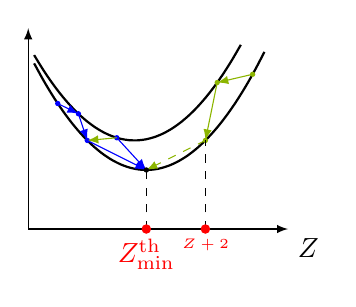
\begin{tikzpicture}[scale=1.5]
    % Ejes (solo el primer cuadrante)
    \draw[-latex] (0,0) -- (2.2,0) node[below right] {\(Z\)};
    \draw[-latex] (0,0) -- (0,1.7) ;
    
    % Parábola (en el primer cuadrante)
    \draw[thick, domain=0.05:2, smooth, variable=\x] 
        plot ({\x}, {(\x-1)^2+0.5}); 
        \draw[thick, domain=0.05:1.8, smooth, variable=\x] 
        plot ({\x}, {(\x-0.9)^2+0.75}); 
    
    % Vértice
    \draw[dashed] (1,0)--(1,0.5);
    \node[red, fill=white] at (1,0) [below] {\(Z^\mathrm{th}_\mathrm{min}\)};
    \draw[red, fill=red] (1,0) circle (1pt); % Punto del vértice
    


    \draw[blue, fill=blue] (0.25,{0.25-1)^2+0.5}) circle (0.5pt);
    \draw[blue, fill=blue] (0.425, {(0.425-0.9)^2+0.75}) circle (0.5pt);
    \draw[blue, fill=blue] (0.5,{0.5-1)^2+0.5}) circle (0.5pt);
    \draw[blue, fill=blue] (0.75, {(0.75-0.9)^2+0.75}) circle (0.5pt);
    
    \draw[applegreen, fill=applegreen] (1.9,{1.9-1)^2+0.5}) circle (0.5pt);
    \draw[applegreen, fill=applegreen] (1.6, {(1.6-0.9)^2+0.75}) circle (0.5pt);
    \draw[applegreen, fill=applegreen] (1.5,{1.5-1)^2+0.5}) circle (0.5pt);

    \draw[blue, thin, -latex] (0.25,{0.25-1)^2+0.5})--(0.425, {(0.425-0.9)^2+0.75});

    \draw[blue, thin, -latex] (0.425, {(0.425-0.9)^2+0.75})--(0.5,{0.5-1)^2+0.5});

    \draw[applegreen, thin, -latex] (0.75, {(0.75-0.9)^2+0.75})--(0.5,{0.5-1)^2+0.5});

    \draw[blue, thin, -latex] (0.75, {(0.75-0.9)^2+0.75})--(1,0.5);
    
    \draw[blue, thin, -latex] (0.5,{0.5-1)^2+0.5})--(1,0.5);
    \draw[applegreen, thin, -latex] (1.9,{1.9-1)^2+0.5})--(1.6,{1.6-0.9)^2+0.75});
    \draw[applegreen, thin, -latex] (1.6,{1.6-0.9)^2+0.75})--(1.5,{1.5-1)^2+0.5});

    \draw[applegreen, dashed,thin, -latex] (1.5,{1.5-1)^2+0.5})--(1,0.5);
    \draw[fill] (1,0.5) circle (0.5pt);

    \draw[dashed] (1.5,0)--(1.5,0.75);
    \node[red, fill=white] at (1.5,0) [below] {\tiny{\(Z+2\)}};
    \draw[red, fill=red] (1.5,0) circle (1pt); % Punto del vértice
\end{tikzpicture}

\end{document}
